\chapter{Binäärihakupuu}

Binäärihakupuu on tietorakenne, joka pitää yllä järjestettyä
alkioiden joukkoa. Binäärihakupuu tarjoaa hajautustaulun tavoin
seuraavat tehokkaat joukon perusoperaatiot:

\begin{itemize}
\item lisää alkio $x$ joukkoon
\item tarkista, onko alkio $x$ joukossa
\item poista alkio $x$ joukosta
\end{itemize}

Lisäksi koska binäärihakupuu säilyttää alkiot järjestyksessä,
siihen voi liittää myös mm. seuraavat tehokkaat operaatiot:

\begin{itemize}
\item etsi joukon pienin/suurin alkio
\item etsi pienin alkiota $x$ suurempi alkio
\item etsi suurin alkiota $x$ pienempi alkio
\end{itemize}

Hajautustaulu \emph{ei} pysty tarjoamaan tällaisia operaatioita
tehokkaasti, joten binäärihakupuu on hyvä valinta, jos näille
operaatioille on tarvetta joukon perusoperaatioiden lisäksi.

Binäärihakupuu on mahdollista toteuttaa niin,
että kaikki sen operaatiot toimivat ajassa $O(\log n)$.
Tämä vaatii, että puu on tasapainotettu, minkä saavuttamiseksi
on monia menetelmiä.
Tässä luvussa tutustumme tarkemmin AVL-puuhun, joka on
yksinkertainen esimerkki tasapainoisesta binääripuusta.
Javan tietorakenteissa taas on käytössä punamusta puu,
joka on vaikeampi toteuttaa mutta tietyissä tilanteissa tehokkaampi.

\section{Taustaa binääripuista}

Binääripuu on puurakenne, joka muodostuu $n$ solmusta.
Puussa ylimpänä on solmu, jota kutsutaan juureksi.
Jokaisella solmulla voi olla vasen ja oikea lapsi,
ja kaikilla solmuilla juurta lukuun ottamatta on yksikäsitteinen vanhempi.
Puun lehtiä ovat solmut, joilla ei ole lapsia.
Binääripuun rakenne on rekursiivinen:
jokainen solmu toimii juurena alipuulle,
joka on myös binääripuu.

\begin{figure}
\center
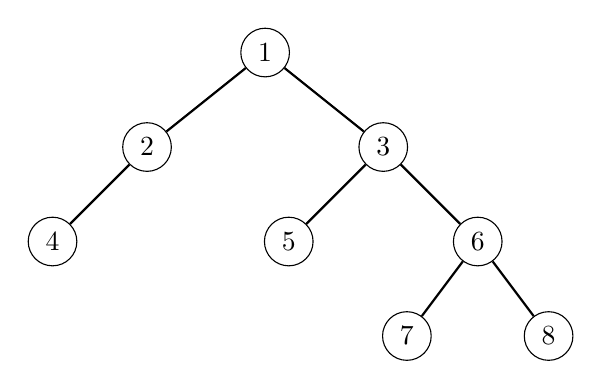
\begin{tikzpicture}[scale=0.6]
\node[draw, circle] (1) at (0,0) {$1$};
\node[draw, circle] (2) at (-2.5,-2) {$2$};
\node[draw, circle] (3) at (2.5,-2) {$3$};
\node[draw, circle] (4) at (-4.5,-4) {$4$};
\node[draw, circle] (5) at (0.5,-4) {$5$};
\node[draw, circle] (6) at (4.5,-4) {$6$};
\node[draw, circle] (7) at (3,-6) {$7$};
\node[draw, circle] (8) at (6,-6) {$8$};
\path[draw,thick,-] (1) -- (2);
\path[draw,thick,-] (1) -- (3);
\path[draw,thick,-] (2) -- (4);
\path[draw,thick,-] (3) -- (5);
\path[draw,thick,-] (3) -- (6);
\path[draw,thick,-] (6) -- (7);
\path[draw,thick,-] (6) -- (8);
\end{tikzpicture}
\caption{Binääripuu, jossa on 8 solmua.}
\label{fig:binpuu}
\end{figure}

Kuvassa \ref{fig:binpuu} on esimerkki binääripuusta, jossa on 8 solmua.
Solmu 1 on puun juuri, ja solmut 4, 5, 7 ja 8 ovat puun lehtiä.
Solmun 3 vasen lapsi on solmu 5, oikea lapsi on solmu 6
ja vanhempi on solmu 1.
Solmun 3 alipuussa ovat solmut 3, 5, 6, 7 ja 8.

Binääripuussa juuren syvyys on 1 ja jokaisen muun solmun syvyys on yhtä
suurempi kuin sen vanhemman syvyys.
Binääripuun korkeus on puolestaan suurin puun solmussa
esiintyvä syvyys.
Esimerkiksi kuvan \ref{fig:binpuu} puun korkeus on 4,
koska solmujen 7 ja 8 syvyys on 4.

Voimme toteuttaa binääripuun Javassa linkitettynä rakenteena.
Seuraava luokkaa vastaa yhtä puussa olevaa solmua:

\begin{code}
public class Node {
    Node left, right;
    int value;

    public Node(Node left, Node right, int value) {
        this.left = left;
        this.right = right;
        this.value = value;
    }
}
\end{code}

Tämän jälkeen voimme määritellä kuvan \ref{fig:binpuu}
binääripuun näin:

\begin{code}
Node node4 = new Node(null, null, 4);
Node node2 = new Node(node4, null, 2);
Node node7 = new Node(null, null, 7);
Node node8 = new Node(null, null, 8);
Node node6 = new Node(node7, node8, 6);
Node node5 = new Node(null, null, 5);
Node node3 = new Node(node5, node6, 3);
Node node1 = new Node(node2, node3, 1);
\end{code}

Voimme käydä läpi binääripuun solmut rekursiivisesti
juuresta alkaen.
Solmujen läpikäyntiin on kolme tavallista järjestystä:

\begin{itemize}
\item \emph{esijärjestys}: käsittelemme ensin solmun, sitten vasemman alipuun
ja lopuksi oikean alipuun
\item \emph{sisäjärjestys}: käsittelemme ensin vasemman alipuun, sitten solmun
ja lopuksi oikean alipuun
\item \emph{jälkijärjestys}: käsittelemme ensin vasemman alipuun,
sitten oikean alipuun ja lopuksi solmun
\end{itemize}

Esimerkiksi kuvan \ref{fig:binpuu} puussa
esijärjestys on $[1,2,4,3,5,6,7,8]$,
sisäjärjes\-tys on $[4,2,1,5,3,7,6,8]$ ja
jälkijärjestys on $[4,2,5,7,8,6,3,1]$.

Seuraava metodi tulostaa binääripuun solmut
sisäjärjestyksessä, kun sille annetaan parametrina
puun juuri.

\begin{code}
void traverse(Node node) {
    if (node == null) return;
    traverse(node.left);
    System.out.println(node.value);
    traverse(node.right);
}
\end{code}

\section{Binäärihakupuun toteutus}

Binäärihakupuu on binääripuu, jossa jokainen solmu vastaa
yhtä joukkoon kuuluvaa alkiota.
Solmut on järjestetty niin, että jokaisessa solmussa
kaikki vasemman alipuun alkiot ovat pienempiä
ja kaikki oikean alipuun alkiot ovat suurempia.
Tämän ominaisuuden ansiosta voimme löytää helposti
alkion puusta aloittamalla haun puun juuresta.

\begin{figure}
\center
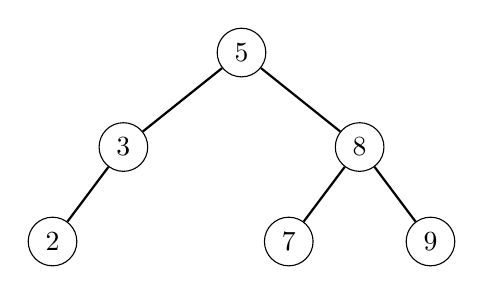
\begin{tikzpicture}[scale=0.6]
\node[draw, circle] (1) at (0,0) {$5$};
\node[draw, circle] (2) at (-2.5,-2) {$3$};
\node[draw, circle] (3) at (2.5,-2) {$8$};
\node[draw, circle] (4) at (-4,-4) {$2$};
\node[draw, circle] (5) at (1,-4) {$7$};
\node[draw, circle] (6) at (4,-4) {$9$};
\path[draw,thick,-] (1) -- (2);
\path[draw,thick,-] (1) -- (3);
\path[draw,thick,-] (2) -- (4);
\path[draw,thick,-] (3) -- (5);
\path[draw,thick,-] (3) -- (6);
\end{tikzpicture}
\caption{Joukkoa $\{2,3,5,7,8,9\}$ vastaava binäärihakupuu.}
\label{fig:bihpuu}
\end{figure}

Kuvassa \ref{fig:bihpuu} on binäärihakupuu,
joka vastaa joukkoa $\{2,3,5,7,8,9\}$.
Esimerkiksi puun juurena on solmu 5,
joten kaikki vasemman alipuun solmut
ovat pienempiä kuin 5 ja kaikki oikean alipuun
solmut ovat suurempia kuin 5.
Sama ehto pätee kaikissa muissakin puun solmuissa.

\subsection{Puun operaatiot}

Seuraavaksi käymme läpi, kuinka voimme toteuttaa
haluamamme joukko-operaatiot
binäärihakupuun avulla.
Jokainen operaatio vie aikaa $O(h)$,
missä $h$ on puun korkeus.

\subsubsection{Alkion etsiminen}

Kun haluamme löytää puusta solmun $x$, lähdemme liikkeelle
puun juuresta ja kuljemme rekursiivisesti alaspäin puussa.
Kun olemme solmussa, jonka arvo on $a$,
vaihtoehtoja on kolme.
Jos $a=x$, olemme löytäneet halutun solmun,
jos $a<x$, jatkamme hakua solmun oikeaan lapseen,
ja jos $a>x$, jatkamme hakua solmun vasempaan lapseen.
Kuitenkin jos haluttua lasta ei ole, toteamme,
että solmua $x$ ei esiinny puussa.

\subsubsection{Alkion lisääminen}

Kun haluamme lisätä puuhun solmun $x$, kuljemme ensin
puussa aivan kuin etsisimme solmua $x$.
Sitten kun olemme päässeet solmuun,
jolla ei ole lasta, johon meidän tulisi edetä,
lisäämme solmun $x$ tällaiseksi lapseksi.

\begin{figure}
\center
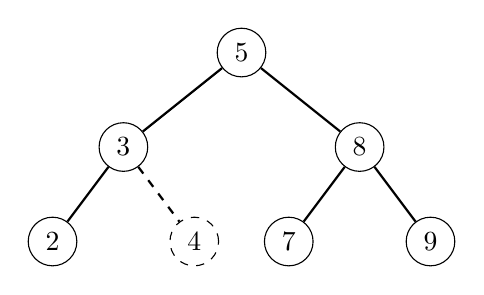
\begin{tikzpicture}[scale=0.6]
\node[draw, circle] (1) at (0,0) {$5$};
\node[draw, circle] (2) at (-2.5,-2) {$3$};
\node[draw, circle] (3) at (2.5,-2) {$8$};
\node[draw, circle] (4) at (-4,-4) {$2$};
\node[draw, circle] (5) at (1,-4) {$7$};
\node[draw, circle] (6) at (4,-4) {$9$};
\node[draw, circle, dashed] (7) at (-1,-4) {$4$};
\path[draw,thick,-] (1) -- (2);
\path[draw,thick,-] (1) -- (3);
\path[draw,thick,-] (2) -- (4);
\path[draw,thick,-] (3) -- (5);
\path[draw,thick,-] (3) -- (6);
\path[draw,thick,dashed,-] (2) -- (7);
\end{tikzpicture}
\caption{Alkion 4 lisääminen joukkoon $\{2,3,5,7,8,9\}$.}
\label{fig:bihpu2}
\end{figure}

Kuva \ref{fig:bihpu2} näyttää, kuinka lisäämme alkion 4
joukkoon $\{2,3,5,7,8,9\}$.
Kun haemme puusta solmua 4, päädymme solmuun 3,
jolla ei ole oikeaa lasta.
Niinpä lisäämme solmun 4 solmun 3 oikeaksi lapseksi.

\subsubsection{Alkion poistaminen}

Kun haluamme poistaa puusta solmun $x$, etsimme ensin
solmun $x$ tavalliseen tapaan.
Jos solmulla $x$ ei ole lapsia, poistamme sen vain puusta.
Jos solmulla $x$ on yksi lapsi, korvaamme solmun $x$
sen lapsella.
Jos kuitenkin solmulla $x$ on kaksi lasta,
tilanne on hankalampi.
Tällöin etsimme puusta solmusta $x$ seuraavan
suuremman alkion $y$ (pian kuvattavalla tavalla), vaihdamme keskenään
solmujen $x$ ja $y$ arvot,
ja poistamme sitten solmun $y$.
Solmulla $y$ ei voi olla kahta lasta, joten poistaminen on helppoa.

\begin{figure}
\center
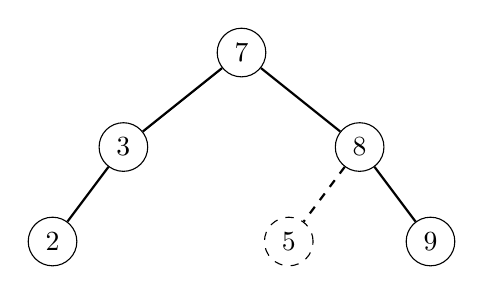
\begin{tikzpicture}[scale=0.6]
\node[draw, circle] (1) at (0,0) {$7$};
\node[draw, circle] (2) at (-2.5,-2) {$3$};
\node[draw, circle] (3) at (2.5,-2) {$8$};
\node[draw, circle] (4) at (-4,-4) {$2$};
\node[draw, circle, dashed] (5) at (1,-4) {$5$};
\node[draw, circle] (6) at (4,-4) {$9$};
\path[draw,thick,-] (1) -- (2);
\path[draw,thick,-] (1) -- (3);
\path[draw,thick,-] (2) -- (4);
\path[draw,thick,-,dashed] (3) -- (5);
\path[draw,thick,-] (3) -- (6);
\end{tikzpicture}
\caption{Alkion 5 poistaminen joukosta $\{2,3,5,7,8,9\}$.}
\label{fig:bihpu3}
\end{figure}


Kuva \ref{fig:bihpu3} näyttää, kuinka poistamme joukosta $\{2,3,5,7,8,9\}$
alkion 5, joka vastaa binäärihakupuun juurta.
Solmun seuraava suurempi alkio on 7,
joten vaihdamme keskenään arvot 5 ja 7.
Tämän jälkeen meidän on helppoa poistaa solmu puusta.

\subsubsection{Pienin/suurin alkio}

Löydämme puun pienimmän alkion lähtemällä liikkeelle
puun juuresta ja siirtymällä vasempaan lapseen niin
kauan kuin tämä on mahdollista.
Solmu, johon päädymme lopulta, on puun pienin alkio.
Vastaavalla tavalla löydämme suurimman alkion
etenemällä koko ajan oikealle juuresta.

\subsubsection{Seuraava suurempi alkio}

Jos solmulla on oikea lapsi, siirrymme ensin solmusta oikealle
ja sitten vasemmalle niin kauan kuin mahdollista.
Muuten kuljemme solmusta ylöspäin, kunnes saavumme solmuun,
jonka vasen lapsi on edellinen lapsi.
Jos tällaista solmua ei ole, solmulla ei ole seuraavaa
suurempaa alkiota.

\subsubsection{Edellinen pienempi alkio}

Menettelemme käänteisesti edelliseen kohtaan nähden.


\subsection{Puun tasapainottaminen}

\section{Javan rakenteet}

\subsection{\texttt{TreeSet}-rakenne}

\subsection{\texttt{TreeMap}-rakenne}

\section{Esimerkki: }

\section{Tehokkuusvertailu}